\section{am::mate$<$ R $>$ Class Template Reference}
\label{classam_1_1mate}\index{am::mate@{am::mate}}
Mates a host function with the mate function object.  


{\tt \#include $<$mate.hpp$>$}

Inherits {\bf am::detail::mate\_\-base}.

Inheritance diagram for am::mate$<$ R $>$:\begin{figure}[H]
\begin{center}
\leavevmode
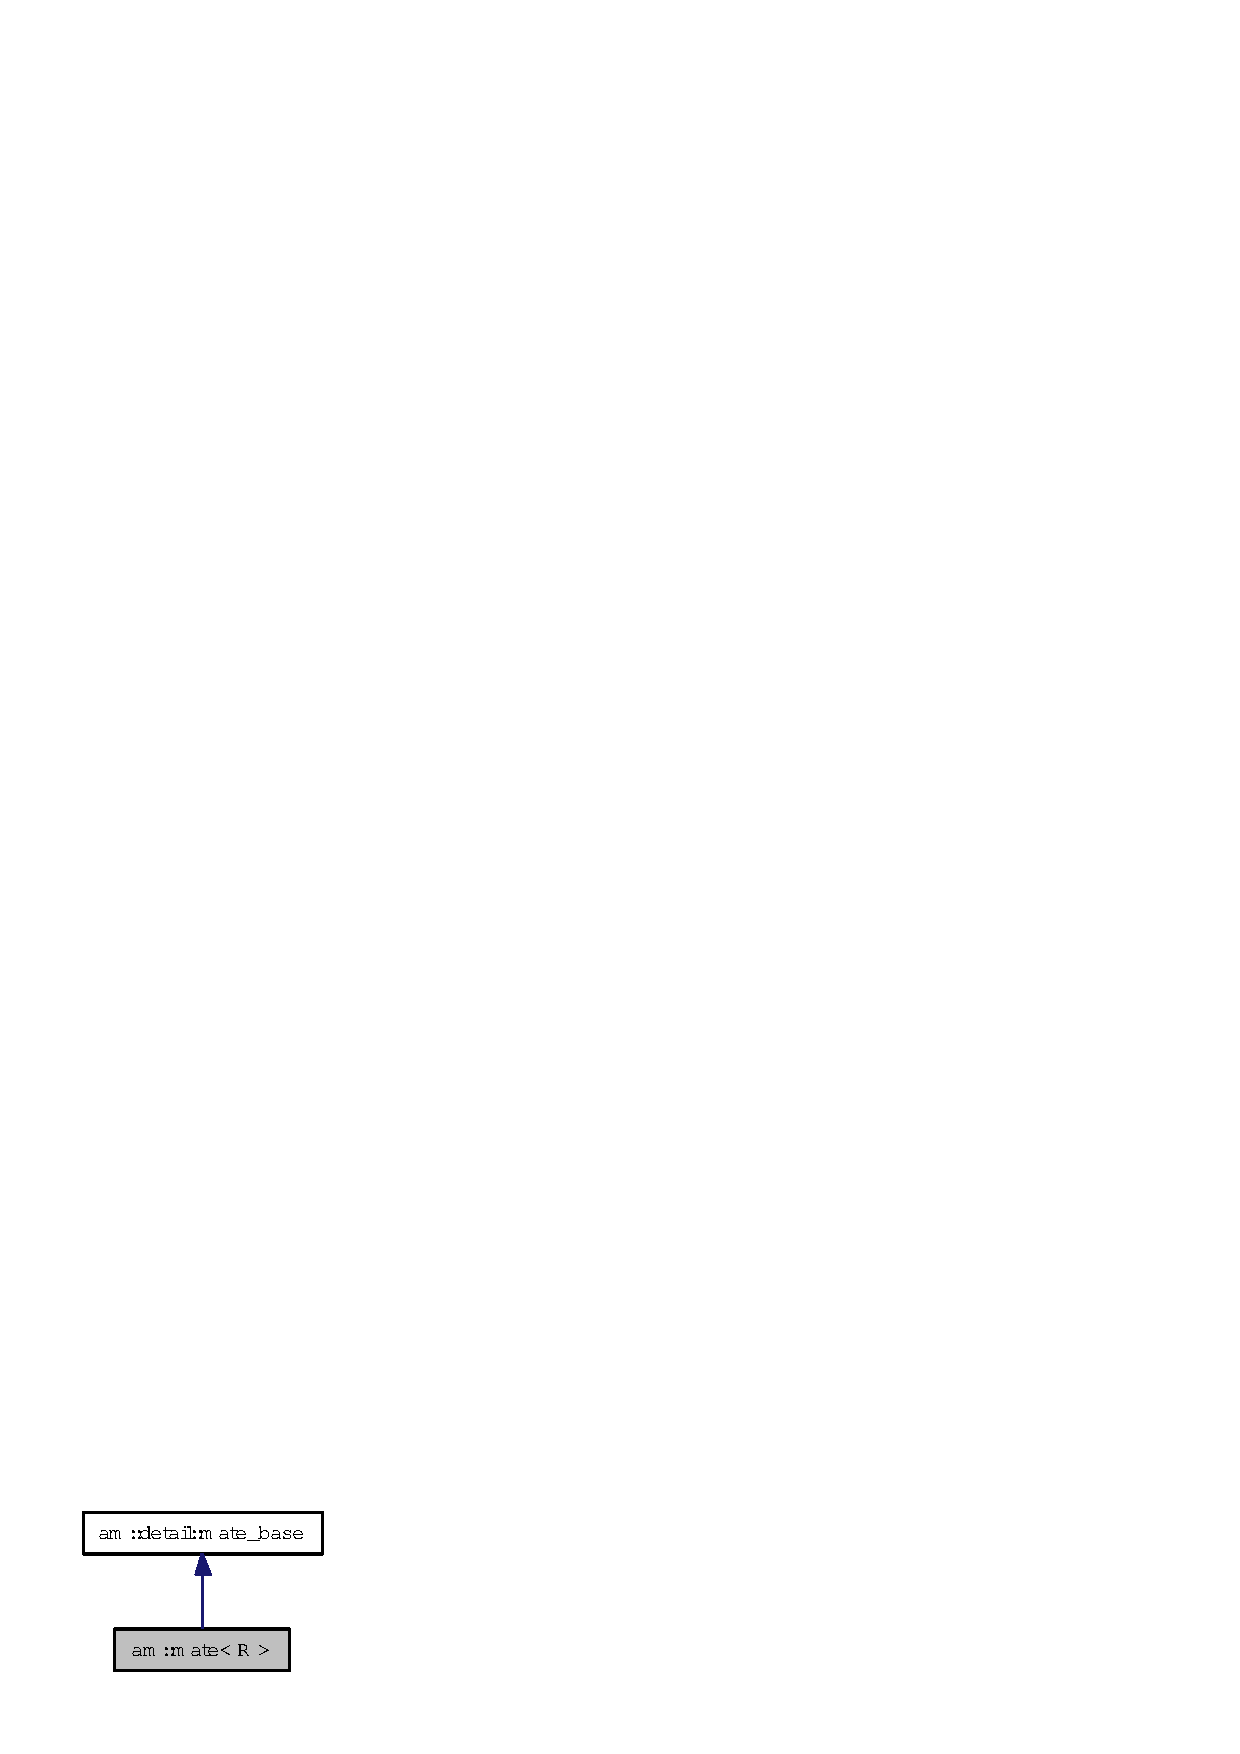
\includegraphics[width=79pt]{classam_1_1mate__inherit__graph}
\end{center}
\end{figure}
Collaboration diagram for am::mate$<$ R $>$:\begin{figure}[H]
\begin{center}
\leavevmode
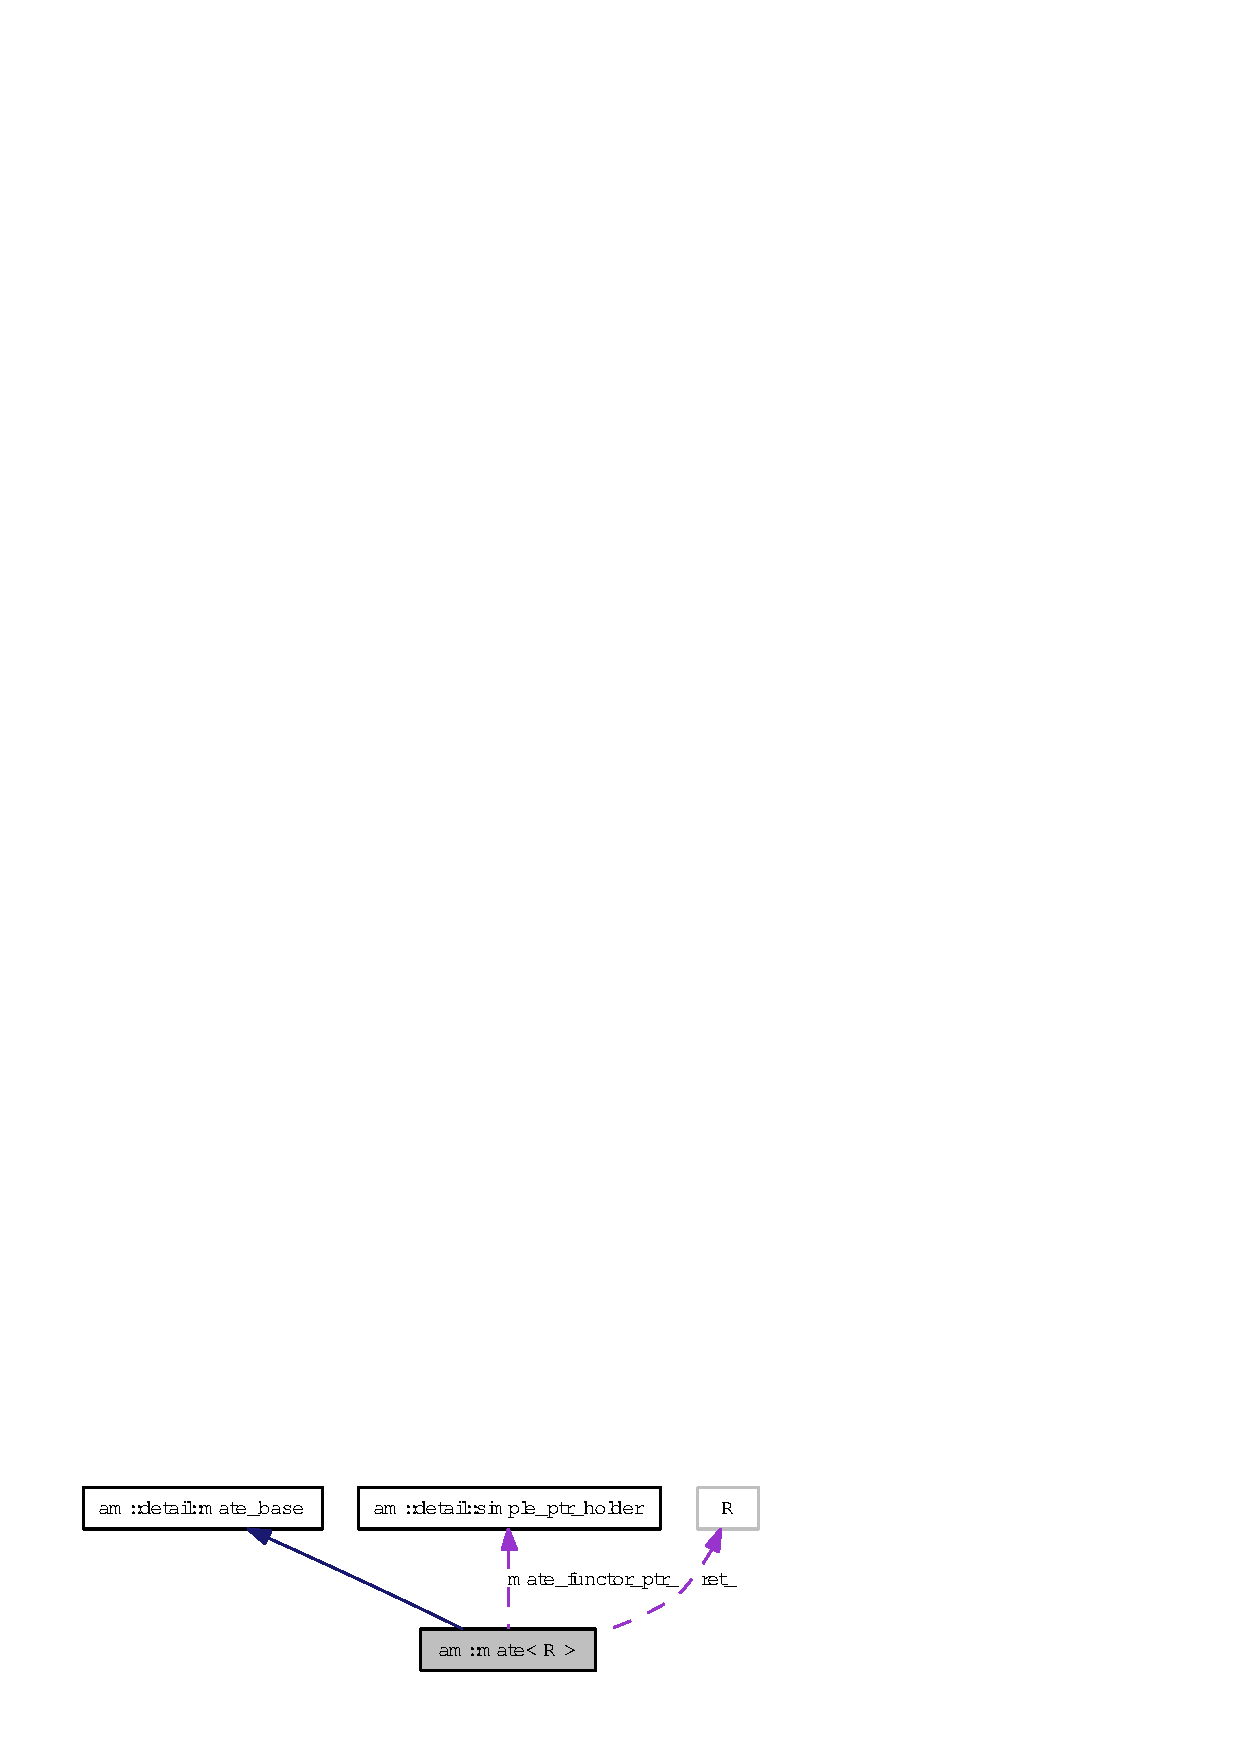
\includegraphics[width=185pt]{classam_1_1mate__coll__graph}
\end{center}
\end{figure}
\subsection*{Public Member Functions}
\begin{CompactItemize}
\item 
template$<$class T$>$ {\bf mate} (R ret, T mate\_\-functor)
\item 
template$<$class T, class C$>$ {\bf mate} (R ret, T mate\_\-functor, C mate\_\-if)
\item 
{\bf $\sim$mate} ()
\item 
void {\bf run\_\-mate} (bool delete\_\-mate\_\-now=false)
\item 
void {\bf dismiss\_\-mate} (bool delete\_\-mate\_\-now=false)
\item 
{\bf operator R} () const
\end{CompactItemize}
\subsection*{Private Types}
\begin{CompactItemize}
\item 
typedef void($\ast$) \textbf{typeless\_\-mate\_\-stub} (void $\ast$, R)\label{classam_1_1mate_ee9347452cd87f7f0fc174ee8eece9de}

\end{CompactItemize}
\subsection*{Private Member Functions}
\begin{CompactItemize}
\item 
{\bf mate}$<$ R $>$ \& {\bf operator=} ({\bf mate}$<$ R $>$ const \&)\label{classam_1_1mate_a2cffaf7bd7a21ba6671e3eb7b7290be}

\begin{CompactList}\small\item\em Restrict assignment. \item\end{CompactList}\end{CompactItemize}
\subsection*{Private Attributes}
\begin{CompactItemize}
\item 
R {\bf ret\_\-}\label{classam_1_1mate_96d8f086acedaaba49fa8dda704c6e68}

\begin{CompactList}\small\item\em Return of the host function. \item\end{CompactList}\item 
{\bf detail::simple\_\-ptr\_\-holder} {\bf mate\_\-functor\_\-ptr\_\-}\label{classam_1_1mate_dac8b8d494662bc0c5cf0a9f0586a465}

\begin{CompactList}\small\item\em Mate functoion object. \item\end{CompactList}\item 
typeless\_\-mate\_\-stub {\bf mate\_\-stub\_\-}\label{classam_1_1mate_72f5837ec74e2e14cdb93f69031b95be}

\begin{CompactList}\small\item\em Typeless mate function object invoker. \item\end{CompactList}\end{CompactItemize}
\subsection*{Classes}
\begin{CompactItemize}
\item 
struct {\bf typed\_\-}
\end{CompactItemize}


\subsection{Detailed Description}
\subsubsection*{template$<$class R$>$ class am::mate$<$ R $>$}

Mates a host function with the mate function object. 

Mates (associates) the result of the host function with the mate function object so that the associated mate function object is called int its destructor automatically when it goes out of scope. 



\subsection{Constructor \& Destructor Documentation}
\index{am::mate@{am::mate}!mate@{mate}}
\index{mate@{mate}!am::mate@{am::mate}}
\subsubsection{\setlength{\rightskip}{0pt plus 5cm}template$<$class R$>$ template$<$class T$>$ {\bf am::mate}$<$ R $>$::{\bf mate} (R {\em ret}, T {\em mate\_\-functor})\hspace{0.3cm}{\tt  [inline]}}\label{classam_1_1mate_52e89c5bf178aff995128a241fc6c3cc}


Constructor.

\begin{Desc}
\item[Parameters:]
\begin{description}
\item[\mbox{$\leftarrow$} {\em ret}]Specifies the return of the host function. \item[\mbox{$\leftarrow$} {\em mate\_\-functor}]Specifies the mate function object which will be called in the destructor. It should be a unary function object which accept {\em ret\/} as its argument.\end{description}
\end{Desc}
\begin{Desc}
\item[Precondition:]Host function should not throw an exception. \end{Desc}
\index{am::mate@{am::mate}!mate@{mate}}
\index{mate@{mate}!am::mate@{am::mate}}
\subsubsection{\setlength{\rightskip}{0pt plus 5cm}template$<$class R$>$ template$<$class T, class C$>$ {\bf am::mate}$<$ R $>$::{\bf mate} (R {\em ret}, T {\em mate\_\-functor}, C {\em mate\_\-if})\hspace{0.3cm}{\tt  [inline]}}\label{classam_1_1mate_0992eeb490ba954833e27e0935861b5a}


Constructor.

\begin{Desc}
\item[Parameters:]
\begin{description}
\item[\mbox{$\leftarrow$} {\em ret}]Specifies the return of the host function. \item[\mbox{$\leftarrow$} {\em mate\_\-functor}]Specifies the mate function object which will be called in the destructor. It should be an unary function object which accept {\em ret\/} as its argument. \item[\mbox{$\leftarrow$} {\em mate\_\-if}]Specifies the predicate which determines whether or not the specified mate function object will be called in the destructor. It should be an unary predicate which accept {\em ret\/} as its argument. If it return false, no heap memory allocation is even occurred to store the mate function object.\end{description}
\end{Desc}
\begin{Desc}
\item[Precondition:]Host function should not throw an exception. \end{Desc}
\index{am::mate@{am::mate}!~mate@{$\sim$mate}}
\index{~mate@{$\sim$mate}!am::mate@{am::mate}}
\subsubsection{\setlength{\rightskip}{0pt plus 5cm}template$<$class R$>$ {\bf am::mate}$<$ R $>$::$\sim${\bf mate} ()\hspace{0.3cm}{\tt  [inline]}}\label{classam_1_1mate_29cac99d41b0fb1cbd0be3e2c841444c}


Destructor. Calls mate function object. 

\subsection{Member Function Documentation}
\index{am::mate@{am::mate}!run_mate@{run\_\-mate}}
\index{run_mate@{run\_\-mate}!am::mate@{am::mate}}
\subsubsection{\setlength{\rightskip}{0pt plus 5cm}template$<$class R$>$ void {\bf am::mate}$<$ R $>$::run\_\-mate (bool {\em delete\_\-mate\_\-now} = {\tt false})\hspace{0.3cm}{\tt  [inline]}}\label{classam_1_1mate_93fe5fc5abbe71780e7638bde72e1845}


Run mate function object now.

\begin{Desc}
\item[Parameters:]
\begin{description}
\item[\mbox{$\leftarrow$} {\em delete\_\-mate\_\-now}]Specifies whether or not the mate function object will be deallocated after calling the mate function object. If false, the mate function object will be deallocated in the destructor when it goes out of scope. \end{description}
\end{Desc}
\begin{Desc}
\item[Returns:]void. \end{Desc}
\index{am::mate@{am::mate}!dismiss_mate@{dismiss\_\-mate}}
\index{dismiss_mate@{dismiss\_\-mate}!am::mate@{am::mate}}
\subsubsection{\setlength{\rightskip}{0pt plus 5cm}template$<$class R$>$ void {\bf am::mate}$<$ R $>$::dismiss\_\-mate (bool {\em delete\_\-mate\_\-now} = {\tt false})\hspace{0.3cm}{\tt  [inline]}}\label{classam_1_1mate_2ecbeb01954567c013e9322aa5e8e0da}


Dismiss the mate functor.

\begin{Desc}
\item[Parameters:]
\begin{description}
\item[\mbox{$\leftarrow$} {\em delete\_\-mate\_\-now}]Specifies whether or not the mate function object will be deallocated. If false, the mate function object will be deallocated in the destructor when it goes out of scope. \end{description}
\end{Desc}
\begin{Desc}
\item[Returns:]void. \end{Desc}
\index{am::mate@{am::mate}!operator R@{operator R}}
\index{operator R@{operator R}!am::mate@{am::mate}}
\subsubsection{\setlength{\rightskip}{0pt plus 5cm}template$<$class R$>$ {\bf am::mate}$<$ R $>$::operator R () const\hspace{0.3cm}{\tt  [inline]}}\label{classam_1_1mate_5bd50a39a4ed2ee277652d394de0acab}


Implicit conversion. Cast an illusion to make it possible to use a mate instance as if it is a raw variable stored, which is the return of the host function.

\begin{Desc}
\item[Returns:]Copy of the stored raw variable, which is the return of the host function. \end{Desc}


The documentation for this class was generated from the following file:\begin{CompactItemize}
\item 
{\bf mate.hpp}\end{CompactItemize}
